376. В некоторой стране выпустили монеты номиналами 1, 5, 10 рублей, на обратной стороне которых
могут быть изображены корона, замок или орёл. Затем все пятирублёвые и десятирублёвые монеты
с изображением замка вывели из обращения. На столе лежат 6 монет, как показано на картинке.
Отметьте галочкой, какие монеты обязательно нужно перевернуть, чтобы узнать, есть ли среди них
выведенные из обращения.\\
\begin{figure}[ht!]
\center{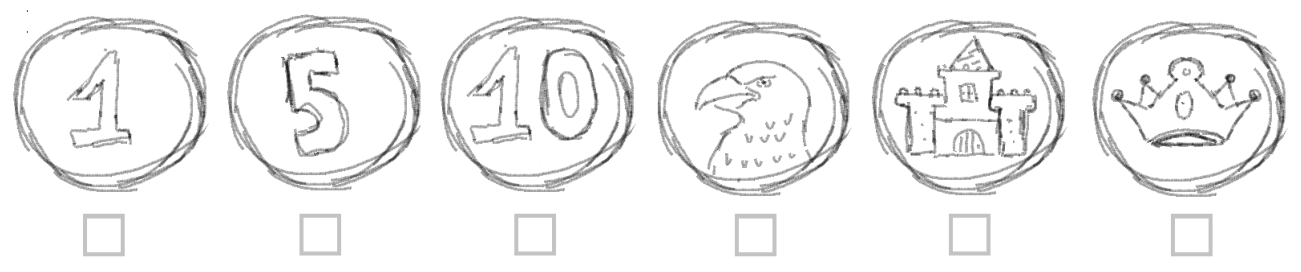
\includegraphics[scale=0.35]{mon1.png}}
\end{figure}\\
